\setcounter{deso}{4}
\begin{name}
	{ÔN TẬP KIỂM TRA CUỐI HỌC KÌ 1 - tp2}
	{TOÁN 10}
	{LỚP TOÁN THẦY PHÁT}
	{\thoigian}
\end{name}
%================================PHẦN I
\caulc
\Opensolutionfile{ans}[ans/0-HK1-CD-4-HoaiDucB-HaNoi-2324-Phan-I]
\begin{ex}%[0D2N2-2]
Điểm nào sau đây thuộc miền nghiệm của hệ bất phương trình $\heva{&x+y+5>0 \\ &x+y+1<0}$?
\choice
{\True $(0;-2)$}
{$(0;2)$}
{$(1;0)$}
{$(0;0)$}
	\loigiai 
{Thay $x=0$, $y=-2$ vào hệ phương trình ta thấy $\heva{&0-2+5>0 \\ &0-2+1<0} \Leftrightarrow \heva{&3>0 \\ &-1<0}$ thỏa mãn.
	}
\end{ex}
\begin{ex}%[0D3H2-2]
	Giá trị lớn nhất của hàm số $y=-3x^2+2x+1$ trên đoạn $[1;3]$ là
	\choice
	{$\dfrac{4}{5}$}
	{$-20$}
	{$\dfrac{1}{3}$}
	{\True $0$}
	\loigiai 
	{Tọa độ đỉnh $I\left(\dfrac{1}{3};\dfrac{4}{3}\right)$. Vì $a=-3<0$ nên hàm số nghịch biến trên $[1;3]$. \\
Ta có $y(1)=0$; $y(3)=-20$. Suy ra $\max\limits_{x\in [1;3]} y=0$ khi $x=1$.		
	}
\end{ex}
\begin{ex}%[0H5H3-5]
	Trên đường thẳng chứa cạnh $BC$ của tam giác $ABC$ lấy một điểm $M$ sao cho $\overrightarrow{MB}=3\overrightarrow{MC}$. Khi đó, đẳng thức nào sau đây đúng?
	\choice
	{$\overrightarrow{AM}=2\overrightarrow{AB}+\overrightarrow{AC}$}
	{$\overrightarrow{AM}=\overrightarrow{AB}-\overrightarrow{AC}$}
	{$\overrightarrow{AM}=\dfrac{1}{2}\left(\overrightarrow{AB}+\overrightarrow{AC}\right)$}
	{\True $\overrightarrow{AM}=-\dfrac{1}{2}\overrightarrow{AB}+\dfrac{3}{2}\overrightarrow{AC}$}
	\loigiai 
	{\begin{center}
			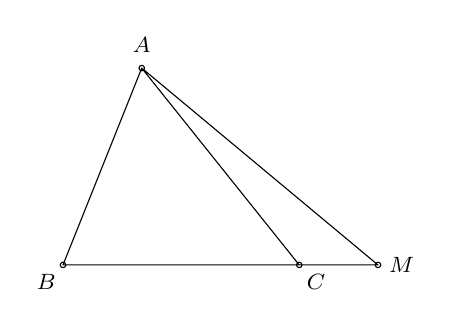
\begin{tikzpicture}[line cap=round, line join=round,font=\footnotesize,>=stealth, scale=1]
				\path (0,0) coordinate (B)
				(3,0) coordinate (C)
				(1,2.5) coordinate (A) (4,0) coordinate (M);
				\draw (B)--(A)--(C)--(B) (C)--(M)--(A);
				\foreach \x/\y in {A/90,B/-135,C/-45,M/0} \draw (\x) circle (1pt)+(\y:0.3) node{$\x$};
			\end{tikzpicture}
	\end{center}
 Ta có 
 \begin{eqnarray*}
 	& & \overrightarrow{MB}=3\overrightarrow{MC}\\
 	&\Leftrightarrow & \overrightarrow{MA}+\overrightarrow{AB}=3\left( \overrightarrow{MA}+\overrightarrow{AC}\right)\\
 	&\Leftrightarrow &-2\overrightarrow{MA}=-\overrightarrow{AB}+3 \overrightarrow{AC}\\
 	&\Leftrightarrow & \overrightarrow{AM}=-\dfrac{1}{2}\overrightarrow{AB}+ \dfrac{3}{2} \overrightarrow{AC}.
\end{eqnarray*}}
\end{ex}
\begin{ex}%[0D3N2-1]
	Cho parabol $(P)\colon y=3x^2-2x+1$. Điểm nào sau đây là đỉnh của $(P)$?
	\choice
	{$I(0;1)$}
	{\True $I\left(\dfrac{1}{3};\dfrac{2}{3}\right)$}
	{$I\left(-\dfrac{1}{3};\dfrac{2}{3}\right)$}
	{$I\left(\dfrac{1}{3};-\dfrac{2}{3}\right)$}
	\loigiai 
{Ta có $a=3$; $b=-2$; $c=1$ và $\Delta=b^2-4ac=(-2)^2-4\cdot3\cdot 1=-8$.\\
Tọa độ đỉnh $I\left(-\dfrac{b}{2a};-\dfrac{\Delta}{4a}\right)$ nên $I\left(\dfrac{1}{3};\dfrac{2}{3}\right)$.	
	}
\end{ex}
\begin{ex}%[0D3H2-3]
	\immini[thm]{Cho hàm số $y=ax^2+bx+c$ có đồ thị như bên. Khẳng định nào sau đây đúng?
	\choice[2]
	{\True $a>0$, $b<0$, $c<0$}
	{$a>0$, $b<0$, $c>0$}
	{$a>0$, $b>0$, $c<0$}
	{$a<0$, $b<0$, $c>0$}}
	{\begin{tikzpicture}[scale=0.65, font=\footnotesize, line join=round,	line cap=round, >=stealth]
			\def\xt{-2} % Hệ số a phải khác 0
			\def\xp{4}
			\def\yd{-4.5}
			\def\yt{1.5}
			\draw[->] (\xt,0) -- (\xp,0) node[below] {$x$};
			\draw[->] (0,\yd) -- (0,\yt) node[left] {$y$};
			\fill (0,0)node[below left]{$O$};
			\clip (\xt,\yd) rectangle (\xp,\yt);
			\draw[samples=100,smooth,domain=-5:5] plot(\x,{(\x)^2-2*(\x)-3});
			\draw[dashed] (1,0)|-(0,-4);
	\end{tikzpicture}}
	\loigiai 
	{Đồ thị hàm số có bề lõm hướng lên trên nên $a>0$.\\
	Trục đối xứng $x=-\dfrac{b}{2a}>0$. Mà $a>0$ nên $b<0$.\\
	Đồ thị hàm số cắt trục tung tại điểm có tung độ âm nên $c<0$.
	}
\end{ex}
\begin{ex}%[0D1H3-3]
	Cho hai tập hợp $A=[-2;7)$, $B=(1;9]$. Tìm $A\cup B$.
	\choice
	{$(1;7)$}
	{\True $[-2;9]$}
	{$[-2;1)$}
	{$(7;9]$}
	\loigiai 
{$A\cup B=[-2;7) \cup (1;9]=[-2;9]$.	
	}
\end{ex}
\begin{ex}%[0D1N2-1]
	Cho tập hợp $A=\big\{x \in \mathbb{N} \mid x \leq 5\big\}$. Tập hợp $A$ viết dưới dạng liệt kê các phần tử là
	\choice
	{$A=\{1;2;3;4\}$}
	{\True $A=\{0;1;2;3;4;5\}$}
	{$A=\{1;2;3;4;5\}$}
	{$A=\{0;1;2;3;4\}$}
	\loigiai 
	{Tập $A=\{0;1;2;3;4;5\}$.	
	}
\end{ex}
\begin{ex}%[0D1N1-3]
	 Lập mệnh đề phủ định của mệnh đề \lq\lq $\forall x \in \mathbb{R} \colon x^2+x+2022>0$\rq\rq.
	\choice
	{\True $\exists x\in\mathbb{R}\colon x^2+x+2022\leq0$}
	{$\forall x\in\mathbb{R}\colon x^2+x+2022<0$}
	{$\forall x\in\mathbb{R}\colon x^2+x+2022\leq0$}
	{$\exists x\in\mathbb{R}\colon x^2+x+2022<0$}
	\loigiai 
	{Mệnh đề phủ định \lq\lq $\exists x \in \mathbb{R}\colon x^2+x+2022\leq0$\rq\rq.		
	}
\end{ex}
\begin{ex}%[0D3N1-2]
	Tập xác định $\mathscr{D}$ của hàm số $y=\dfrac{3x-1}{2x-2}$ là
	\choice
	{$\mathscr{D}=\mathbb{R}$}
	{$\mathscr{D}=[1;+\infty)$}
	{$\mathscr{D}=(1;+\infty)$}
	{\True $\mathscr{D}=\mathbb{R}\setminus\{1\}$}
	\loigiai 
	{Điều kiện $2x-2\ne0 \Leftrightarrow x\ne1$. Suy ra $\mathscr{D}=\mathbb{R}\setminus\{1\}$.	
	}
\end{ex}
\begin{ex}%[0H4N1-1]
	Cho $0^{\circ}<\alpha<90^{\circ}$. Mệnh đề nào sau đây là mệnh đề đúng?
	\choice
	{\True $\cos\left(90^{\circ}-\alpha\right)=\sin\alpha$}
	{$\sin\left(90^{\circ}-\alpha\right)=-\cos\alpha$}
	{$\cot\left(90^{\circ}-\alpha\right)=-\tan\alpha$}
	{$\tan\left(90^{\circ}-\alpha\right)=-\cot\alpha$}
	\loigiai 
	{Ta có $\cos\left(90^{\circ}-\alpha\right)=\sin\alpha$.
	}
\end{ex}
\begin{ex}%[0D3N2-2]
	Khoảng nghịch biến của hàm số $y=x^2-4x+3$ là	
	\choice
	{$(-\infty;5)$}
	{$(-\infty;7)$}
	{\True $(-\infty;2)$}
	{$(-2;+\infty)$}
	\loigiai 
	{Tọa độ đỉnh $I(2;-1)$. Do hệ số $a=1>0$ nên hàm số nghịch biến trên $(-\infty;2)$. 			
	}
\end{ex}
\begin{ex}%[0H5H3-3]
	Cho tam giác $ABC$ và $M$ là điểm thỏa $\overrightarrow{MA}+\overrightarrow{MB}+\overrightarrow{MC}=\overrightarrow{0}$. Mệnh đề nào sau đây đúng?
	\choice
	{$M$ là trung điểm $AB$}
	{\True $M$ là trọng tâm $\triangle ABC$}
	{$M$ trùng $B$}
	{$A$ là trung điểm $MB$}
	\loigiai 
	{Gọi $G$ là trung điểm của tam giác $ABC$ nên ta có
\begin{eqnarray*}
	& & \overrightarrow{MA}+\overrightarrow{MB}+\overrightarrow{MC}=\overrightarrow{0}\\
	&\Leftrightarrow & 3\overrightarrow{MG}+\overrightarrow{GA}+\overrightarrow{GB}+\overrightarrow{GC}=\overrightarrow{0}\\
	&\Leftrightarrow & 3\overrightarrow{MG}=\overrightarrow{0}\\
		&\Leftrightarrow & \overrightarrow{MG}=\overrightarrow{0}.
\end{eqnarray*}
Suy ra $M$ trùng với $G$.\\
 Vậy $M$ là trọng tâm $\triangle ABC$.
	}
\end{ex}
\Closesolutionfile{ans}
%================================PHẦN II
\cauds
\Opensolutionfile{ans}[ans/0-HK1-CD-4-HoaiDucB-HaNoi-2324-Phan-II]
\begin{ex}%[0H5H3-6]
	Cho $\triangle ABC$ vuông cân tại $A$ có $BC=a\sqrt{2}$, $M$ là trung điểm $BC$. 
	\choiceTF 
	{$\left|\overrightarrow{AB}\right|=a\sqrt{2}$}
	{$\left|\overrightarrow{AB}-\overrightarrow{AC}\right|=\dfrac{a \sqrt{2}}{2}$}
	{\True $\left|\overrightarrow{AB}+\overrightarrow{AC}\right|=a\sqrt{2}$}
	{\True $\left|\overrightarrow{AB}+\overrightarrow{BM}-\overrightarrow{BC}\right|=\dfrac{a\sqrt{10}}{2}$}
	\loigiai 
{\begin{center}
			\begin{tikzpicture}[scale=1.0, font=\footnotesize, line join=round, line cap=round, >=stealth]
				\path
				(0,0)coordinate(A)++(0:4)coordinate(C)
				(A)++(90:4)coordinate(B)
				;
				\coordinate (M) at ($(B)!1/2!(C)$);
				\draw (A)--(B)--(C)--cycle (A)--(M)
				;
				\draw pic[draw,angle radius=3mm] {right angle = C--A--B};
				\draw pic[draw,angle radius=3mm] {right angle = A--M--C};
				\foreach \diem/\goc in{A/180,B/90,C/0,M/90}
				\fill[black] (\diem)circle(1pt) ($(\diem)+(\goc:3mm)$)node{$\diem$};
				\end{tikzpicture}
\end{center}
\begin{itemchoice}
			\itemch {\bf Sai}.\\
			Ta có $\triangle ABC$ vuông cân tại $A$ có $BC=a \sqrt{2}$ nên $AB=AC=a$.
			\itemch {\bf Sai}.\\
		$\left|\overrightarrow{AB}-\overrightarrow{AC}\right|=\left|\overrightarrow{BC}\right|=BC=a\sqrt{2}$.
			\itemch {\bf Đúng}.\\
		$\left|\overrightarrow{AB}+\overrightarrow{AC}\right|=
		\left|2\overrightarrow{AM}\right|=2AM=BC=a\sqrt{2}$.
			\itemch {\bf Đúng}.\\
			 $\left|\overrightarrow{AB}+\overrightarrow{BM}-\overrightarrow{BC}\right|=\left|\overrightarrow{AM}-\overrightarrow{BC}\right|$.\\
Ta lại có 	$\left|\overrightarrow{AM}-\overrightarrow{BC}\right|^{2}={\overrightarrow{AM}}^{2}-2\overrightarrow{AM}\cdot \overrightarrow{BC}+{\overrightarrow{BC}}^{2}={\overrightarrow{AM}}^{2}+{\overrightarrow{BC}}^{2}=\left(\dfrac{a\sqrt{2}}{2}\right)^{2}+(a\sqrt{2})^{2}=\dfrac{5a^{2}}{2}$.\\
(Do $M$ là trung điểm $BC$ nên $AM \perp BC \Leftrightarrow \overrightarrow{AM} \cdot \overrightarrow{BC}=\overrightarrow{0}$).\\
Suy ra 	$\left|\overrightarrow{AM}-\overrightarrow{BC}\right|=\dfrac{a\sqrt{10}}{2}$.		 
\end{itemchoice}
}
\end{ex}

\begin{ex}%[0D3V2-2]
	Cho hàm số $ f(x)=x^2+(2m+1)x+m^2-1$ 
	\choiceTF
	{\True Với $m=1$ hàm số đồng biến trên khoảng $\left(-1;+\infty\right)$}
	{Với $m=2$, giá trị nhỏ nhất của hàm số là $-\dfrac{5}{2}$}
	{Với $m>-\dfrac{5}{4}$ thì $f(x)>0 \ \forall x \in \mathbb{R}$}
	{\True Có $2$ giá trị của $m$ để giá trị nhỏ nhất của $f(x)$ trên đoạn $[0;1]$ là $1$}
	\loigiai 
	{\begin{itemchoice}
			\itemch {\bf Đúng}.\\
			Với $m=1$ suy ra $f(x)=x^2+3x$ có $a=1$, $b=3$, $c=0$ và $\Delta=b^2-4ac=9$.\\
			Từ đó suy ra đỉnh $I\left(-\dfrac{3}{2};-\dfrac{9}{4}\right)$.\\
			Do $a=1>0$ nên hàm số đồng biến trên khoảng $\left(-\dfrac{3}{2};+\infty\right)$. 
			\itemch {\bf Sai}.\\
			Với $m=1$ suy ra $f(x)=x^2+5x+3$ có đỉnh $I\left(-\dfrac{5}{2};-\dfrac{13}{4}\right)$.\\
			Do $a=1>0$ nên hàm số đạt giá trị nhỏ nhất bằng $-\dfrac{13}{4}$ khi $x=-\dfrac{5}{2}$. 
			\itemch {\bf Sai}.\\
			Ta có $a=1>0$. Để $f(x)>0$, $\forall x \in \mathbb{R}$ thì $\Delta<0$.\\
			Suy ra $\left(2m+1\right)^{2}-4\left(m^{2}-1\right)<0 \Leftrightarrow 4m+5<0 \Leftrightarrow m<-\dfrac{5}{4}$.
			\itemch {\bf Đúng}.\\
			Ta có $-\dfrac{b}{2a}=\dfrac{-2m-1}{2}$, $\Delta=4m+5$.\\
			Vì $a>0$ nên đồ thị hàm số là một parabol quay bề lõm lên trên và có điểm thấp nhất là đỉnh $I\left(-\dfrac{b}{2a};-\dfrac{\Delta}{4a}\right)$. Từ đó ta xét các trường hợp sau:
		\begin{itemize}
			\item TH1 $.-\dfrac{b}{2a} \in (0;1) \Rightarrow 0<\dfrac{-2m-1}{2}<1 \Rightarrow -\dfrac{3}{2}<m<-\dfrac{1}{2}$ . \hfill (1)\\
			Khi đó $\min\limits_{x\in[0;1]} f(x)=-\dfrac{\Delta}{4a}=\dfrac{-4m-5}{4}$.\\
			Suy ra $\dfrac{-4m-5}{4}=1\Rightarrow m=-\dfrac{9}{4}$ (loại).
			\item TH2 $.-\dfrac{b}{2a} \le 0 \Rightarrow \dfrac{-2m-1}{2}\le 0 \Rightarrow m \ge -\dfrac{1}{2}$ . \hfill (2)\\
			Khi đó $\min\limits_{x\in[0;1]}f(x)=f(0)=m^{2}-1$.\\
			Suy ra $m^{2}-1=1\Rightarrow \hoac{&m=\sqrt{2}\\&m=-\sqrt{2}}$, đối chiếu với điều kiện (2) ta thấy $m=\sqrt{2}$ thỏa mãn.
			\item TH3 $.-\dfrac{b}{2a} \ge 1 \Rightarrow \dfrac{-2m-1}{2}\ge 1 \Rightarrow m \le -\dfrac{3}{2}$. \hfill (3)\\
			Khi đó $\min\limits_{x\in[0;1]} f(x)=f(1)=m^{2}+2m+1$.\\
			Suy ra $m^{2}+2m+1=1\Rightarrow \hoac{&m=0\\&m=-2}$, đối chiếu với điều kiện (3) ta thấy $m=-2$ thỏa mãn.
		\end{itemize}
	Vậy có $2$ giá trị của $m$ thỏa mãn yêu cầu bài toán.
		\end{itemchoice}
	}
\end{ex}
\Closesolutionfile{ans}
%================================PHẦN III
\caukq
\Opensolutionfile{ans}[ans/0-HK1-CD-4-HoaiDucB-HaNoi-2324-Phan-III]
\begin{ex}%[De-chuan-hoa-so-1]%[Diamond]%[0D1V3-5]
Trong một khoảng thời gian nhất định tại một địa phương, Đài khí tượng thủy văn đã thống kê được: Số ngày có mưa: 10 ngày; số ngày có gió to: 8 ngày; số ngày lạnh: 6 ngày; số ngày có mưa và gió to: 5 ngày; số ngày mưa và lạnh: 4 ngày; số ngày lạnh và có gió to: 3 ngày; số ngày có mưa, lạnh và có gió to: 1 ngày. Hỏi trong khoảng thời gian đó, địa phương trên có bao nhiêu ngày có thời tiết xấu (có mưa hoặc gió to hoặc lạnh)?
\shortans[]{$13$}
\loigiai{
Gọi $A$, $B$, $C$ lần lượt là tập hợp ngày có mưa, ngày có gió to, ngày lạnh.
Theo giả thiết đề bài cho, ta có biểu đồ Ven
\begin{center}
\begin{tikzpicture}[scale=0.7, font=\footnotesize, line join=round, line cap=round, >=stealth]
\path
(0,0) coordinate (A)
(3,0) coordinate (B)
(3,3) coordinate (C)
(0,3) coordinate (D)
($(A)!{1/4}!(C)$) coordinate (M)
($(C)!{1/2}!(D)$) coordinate (N)
;
\draw[thick,blue] (0,0) ellipse (2.8cm and 2cm);
\draw[thick,red] (4,0) ellipse (2.8cm and 2cm);
\draw[thick,black] (2,-2.2) ellipse (2.8cm and 2cm);
\draw (2,0.5) node[]{$4$} (2,-0.7) node[]{$1$} (0.7,-1.25) node[]{$3$} (3.5,-1.25) node[]{$2$} ;
\draw (-2.1,1.5) node[left]{$A$} (6.1,1.5) node[right]{$B$}
(4,-4) node[right]{$C$};
\end{tikzpicture}
\end{center}
Số ngày chỉ có mưa là $10-4-3-1 = 2$ ngày.  \\
Số ngày chỉ có gió to là $8-4-2-1 = 1$ ngày.  \\
Số ngày chỉ lạnh là $6-3-2-1 = 0$ ngày.  \\
Vậy số ngày có thời tiết xấu là $2+1+0+4+3+2+1 = 13$ ngày.
}
\end{ex}
\begin{ex}%[0D3H2-1]
	Parabol $y=ax^2+bx+c$ đi qua $A(0;-1)$, $B(1;-1)$, $C(-1;1)$. Tích $abc$ bằng bao nhiêu?
	\shortans[]{$1$} 
	\loigiai{Do	Parabol $y=a x^2+b x+c$ đi qua $3$ điểm $A(0;-1)$, $B(1;-1)$, $C(-1;1)$ nên ta có hệ phương trình sau 
$\heva{&c=-1\\&a+b+c=-1\\&a-b+c=1} \Rightarrow \heva{&c=-1\\&a=1\\&b=-1.}$\\
Vậy tích $abc=1$.
	}
\end{ex}
\begin{ex}%[0H4H1-3]
	Cho $\sin\alpha=\dfrac{1}{3}$. Tính giá trị của $P=3\sin^2\alpha+\cos^2\alpha-\dfrac{2}{9}$.
	\shortans[]{$1$} 
	\loigiai{
		Ta có $\sin ^2 \alpha+\cos ^2 \alpha=1 \Leftrightarrow \cos ^2 \alpha =1-\left(\dfrac{1}{3}\right)^{2}=\dfrac{8}{9}$.\\
		Suy ra $P=3 \sin ^2 \alpha+\cos ^2 \alpha-\dfrac{2}{9}=3 \cdot \left(\dfrac{1}{3}\right)^{2}+\dfrac{8}{9}-\dfrac{2}{9}=\dfrac{11}{9}-\dfrac{2}{9}=1$.
}
\end{ex}

\begin{ex}%[0D7V2-6]
	Cho hàm số $y=\dfrac{x+1}{x^2-2(m+1)x+m^2+2m}$. Tập hợp tất cả các giá trị của $m$ để hàm số xác định trên $[0;1)$ là $T=(-\infty;a) \cup[b;c) \cup[d;+\infty)$. Tính $P=a+b+c+d$.
	\shortans[]{$-2$} 
	\loigiai{
		Để hàm số xác định trên $[0;1)$ thì $x^2-2(m+1)x+m^2+2 \ne 0$, $\forall x \in [0;1)$.\\
		Suy ra $(x-m)(x-m-2) \ne 0$, $\forall x \in [0;1) \Leftrightarrow \hoac{&\heva{&m+2 \ge 1 \\& m<0}\\&m \ge 1\\&m+2<0} \Leftrightarrow \hoac{&-1 \le m <0\\& m \ge 1\\ &m<-2.}$\\
		$\Rightarrow T=(-\infty;-2) \cup[-1;0) \cup[1;+\infty)$.\\
		 Vậy $P=a+b+c+d=-2-1+0+1=-2$.
	}
\end{ex}
\begin{ex}%[0H5V3-5]
	Cho tam giác $\mathrm{ABC}$.
	Gọi $I$, $J$ là hai điểm được xác định bởi $\overrightarrow{IA}=2 \overrightarrow{IB}$, $3\overrightarrow{JA}+2\overrightarrow{JC}=\overrightarrow{0}$. Đường thẳng $I J$ qua trọng tâm $G$ của tam giác $\triangle ABC$. Biết rằng $\overrightarrow{IJ}=a \overrightarrow{AB}+b \overrightarrow{AC}$. Tính $2a-5b$.
	\shortans[]{$-6$} 
	\loigiai{
Ta có $\overrightarrow{IA}=2 \overrightarrow{IB} \Leftrightarrow \overrightarrow{IA}=2\overrightarrow{IA}+2 \overrightarrow{AB} \Leftrightarrow \overrightarrow{AI}=2\overrightarrow{AB}$.\\
Lại có
\[3 \overrightarrow{JA}+2 \overrightarrow{JC}=\overrightarrow{0} \Leftrightarrow 3 \overrightarrow{JA}+2 \overrightarrow{JA} + 2\overrightarrow{AC}=\overrightarrow{0} \Leftrightarrow 5\overrightarrow{JA}+2\overrightarrow{AC}=\overrightarrow{0} \Leftrightarrow 5\overrightarrow{AJ}=2\overrightarrow{AC} \Leftrightarrow \overrightarrow{AJ}=\dfrac{2}{5}\overrightarrow{AC}.\]
Từ đó suy ra $\overrightarrow{IJ}=\overrightarrow{AJ}-\overrightarrow{AI}=-2\overrightarrow{AB}+\dfrac{2}{5}\overrightarrow{AC}$.\\
Vậy $2a-5b=2\cdot (-2)-5 \cdot \dfrac{2}{5}=-6$.
	}
\end{ex}
\Closesolutionfile{ans}
% \begin{indapan}
% 	{ans/0-HK1-CD-4-HoaiDucB-HaNoi-2324}
% \end{indapan}

\TL
\begin{ex}%[10-11-12EX-HK1-2425]%[Huỳnh Xuân Tín]%[0D7V3-1]
Giải phương trình 
\begin{enumerate}
	\item $\sqrt{x^2-x+1}=\sqrt{x^2+x-3}$;
	\item $\sqrt{2x+3}-\sqrt{x-1}=1$.
\end{enumerate}
\loigiai{
\begin{enumerate}
	\item Ta có
\begin{eqnarray*}
& & \sqrt{x^2-x+1}=\sqrt{x^2+x-3}\\
&\Rightarrow & x^2-x+1=x^2+x-3\\
&\Rightarrow& x=2.
\end{eqnarray*}
Thử lại ta thấy $\sqrt{2^2-2+1}=\sqrt{2^2+2-3}$ đúng nên $x=2$ là nghiệm phương trình đã cho.\\
Vậy tập nghiệm phương trình trên là $S=\{2\}$.
	\item Ta có
\begin{eqnarray*}
& & \sqrt{2x+3}-\sqrt{x-1}=1\\
&\Rightarrow & \sqrt{2x+3}=1+\sqrt{x-1}\\
&\Rightarrow & 2x+3=1+2\sqrt{x-1}+x-1\\
&\Rightarrow & x+3=2\sqrt{x-1}\\
&\Rightarrow & x^2+6x+9=4(x-1)\\
&\Rightarrow & x^2+2x+13=0.
\end{eqnarray*}
Phương trình vô nghiệm.\\
Vậy phương trình đã cho vô nghiệm.
\end{enumerate}
}
\end{ex}
\begin{ex}%[0H5C4-7]%[CTST - Lớp 10 - Ôn tập cuối học kì 1 - Đề 4]%[Phạm Văn Long]
Một chất điểm ở vị trí điểm $O$ chịu tác động bởi ba lực $\vec{F}_1, \vec{F}_2, \vec{F}_3$ có độ lớn là $F_1=6$N, $F_2=4$N, $F_3=2\sqrt{5}$N, góc tạo bởi hai lực $\vec{F}_1$ và $\vec{F}_3$ là $\alpha=60^{\circ}$ (tham khảo hình vẽ). Hỏi chất điểm trên phải chịu tác động hợp lực có độ lớn là bao nhiêu Newton N? (làm tròn đến hàng phần trăm).
\begin{center}
\begin{tikzpicture}[=>stealth,line join=round,line cap=round,thick, font=\footnotesize, scale=.9]
\path
(0,0)node[above]{$\vec{F}_2$}coordinate (F2)
(8,0)node[above]{$\vec{F}_1$}coordinate (F1)
(5,-3)node[left]{$\vec{F}_3$}coordinate (F3);
\coordinate (O) at ($(F2)!0.4!(F1)$);
\draw[red,->] (O)--(F2);
\draw[->] (O)--(F1);
\draw[blue,->] (O)--(F3);
\fill[red,black] (O)node[above]{$O$} circle (1pt);
\end{tikzpicture}
\end{center}
\shortans{5,74}
%Hình vẽ
\loigiai{
\begin{center}
\begin{tikzpicture}[=>stealth,line join=round,line cap=round,thick, font=\footnotesize, scale=1.0]
\path
(0,0)node[above]{$\vec{F}_2$}coordinate (F2)
(8,0)node[above]{$\vec{F}_1$}coordinate (F1)
(5,-3)node[above left]{$\vec{F}_3$}coordinate (F3)
(3.2,-3)node[below]{$F$} coordinate (F)
(5,-3)node[below]{$C$};
\coordinate (O) at ($(F2)!0.4!(F1)$);
\path
(F3)++(0:4.8)coordinate (B)node[below]{$B$}
(B)++(0:-3.2)coordinate (E)node[below]{$E$}
(F3)++(90:3)coordinate (G)node[above]{$G$};
\draw (B)node[right]{$\vec{F}_1+\vec{F}_3$} (F1)node[right]{$A$} (F2)node[left]{$D$};
\draw[red,->] (O)--(F2);
\draw[->] (O)--(F1);
\draw[blue,->] (O)--(F3);
\draw[->] (O)--(E);
\draw[dashed] (F3)--(B)--(F1) (O)--(B) (O)--(F)--(F3) (F2)--(E) (F3)--(G);
\fill[black] (O)node[above]{$O$} circle (1.2pt) (F)circle (1.2pt) (F3)circle (1.2pt) (B)circle (1.2pt) (F1)circle (1.2pt) (F2)circle (1.2pt) (G)circle (1.2pt) (E)circle (1.2pt);
\end{tikzpicture}
\end{center}
Ta dựng hình bình hành $OABC$, suy ra $\overrightarrow{OB}=\vec{F}_1+\vec{F}_3$.\\
Tương tự, ta dựng hình bình hành $ODEB$, suy ra $\overrightarrow{OE}=\vec{F}_1+\vec{F}_2+\vec{F}_3$.\\
Hợp lực tác động lên chất điểm $O$ là độ lớn của vectơ $\overrightarrow{OE}$.\\
Dựng tam giác $O G C$ vuông tại $G$, ta có
\[\cos \alpha=\dfrac{O G}{O C} \Rightarrow O G=O C \cdot \cos \alpha=\sqrt{5}.\]
Suy ra $F C=O G=\sqrt{5}$.\\
Ta có $C E=C B-E B=O A-O D=2, E F=F C+C E=\sqrt{5}+2$.\\
Khi đó $O F=\sqrt{O C^2-F C^2}=\sqrt{(2 \sqrt{5})^2-(\sqrt{5})^2}=\sqrt{15}$.\\
Do đó, $O E=\sqrt{O F^2+F E^2}=\sqrt{15+(2+\sqrt{5})^2}=\sqrt{24+4 \sqrt{5}} \approx 5{,}74$.\\
Vậy, vật chịu tác động một hợp lực có độ lớn là $5{,}74$(N).
}
\end{ex}
\begin{ex}%[0D3C2-6]
Dây truyền đỡ trên cầu treo có dạng parabol $ACB$ như hình vẽ.
\begin{center}
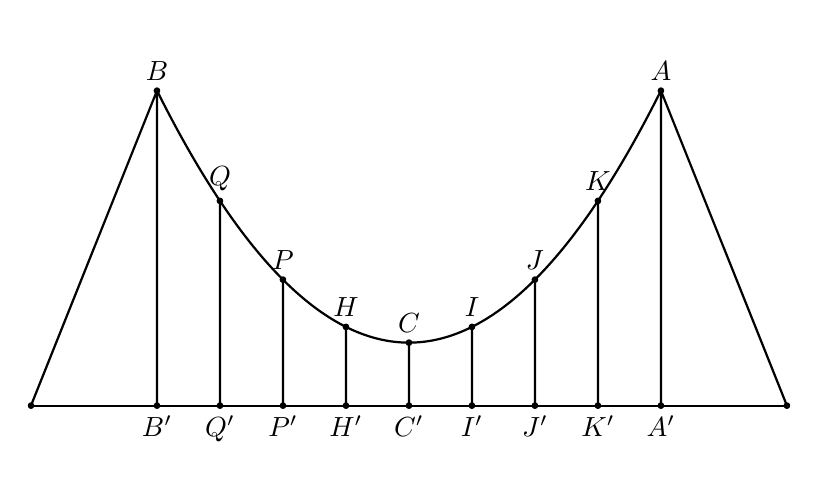
\begin{tikzpicture}[line join=round, line cap=round,>=stealth,thick,scale=.8]
\tikzset{label style/.style={font=\footnotesize}}
\draw[-] (-6,0)--(6,0);
\draw (1,0)--(1,1.25) (-1,0)--(-1,1.25) (-2,0)--(-2,2) (2,0)--(2,2)
(-3,0)--(-3,3.25) (3,0)--(3,3.25) (-4,0)--(-4,5) (4,0)--(4,5)
(-6,0)--(-4,5) (6,0)--(4,5) (0,0)--(0,1);
\draw (0,1) circle (1pt)node [above] {$C$} (0,0) circle (1pt) node [below] {$C'$};
\draw (1,0) circle (1pt)node [below] {$I'$} (1,1.25) circle (1pt) node [above] {$I$};
\draw (-1,0) circle (1pt)node [below] {$H'$} (-1,1.25) circle (1pt) node [above] {$H$};
\draw (-2,0) circle (1pt)node [below] {$P'$} (-2,2) circle (1pt) node [above] {$P$};
\draw (2,0) circle (1pt)node [below] {$J'$} (2,2) circle (1pt) node [above] {$J$};
\draw (-3,0) circle (1pt)node [below] {$Q'$} (-3,3.25) circle (1pt) node [above] {$Q$};
\draw (3,0) circle (1pt)node [below] {$K'$} (3,3.25) circle (1pt) node [above] {$K$};
\draw (-4,0) circle (1pt)node [below] {$B'$} (-4,5) circle (1pt) node [above] {$B$};
\draw (4,0) circle (1pt)node [below] {$A'$} (4,5) circle (1pt) node [above] {$A$};
\draw (-6,0) circle (1pt) (6,0) circle (1pt);
\begin{scope}
\clip (-4,-1) rectangle (4,6);
\draw[samples=200,domain=-4:4,smooth,variable=\x] plot (\x,{0.25*(\x)^2+1});
\end{scope}
\end{tikzpicture}
\end{center}
Đầu, cuối của dây được gắn vào các điểm $A$, $B$ trên mỗi trục $AA'$ và $BB'$ với độ cao $30$ m. Chiều dài đoạn $A'B'$ trên nền cầu bằng $200$ m. Độ cao ngắn nhất của dây truyền trên cầu là $CC'=5$ m. Gọi $Q',P',H',O',I',J',K'$ là các điểm chia đoạn $A'B'$ thành các phần bằng nhau. Các thanh thẳng đứng nối nền cầu với đáy dây truyền: $QQ',PP',HH',CC',II',JJ',KK'$ gọi là các dây cáp treo. Vậy tổng độ dài của các dây cáp treo là bao nhiêu (làm tròn đến hàng phần chục)?
% \shortans{$78{,}8$}
\loigiai{
\begin{center}
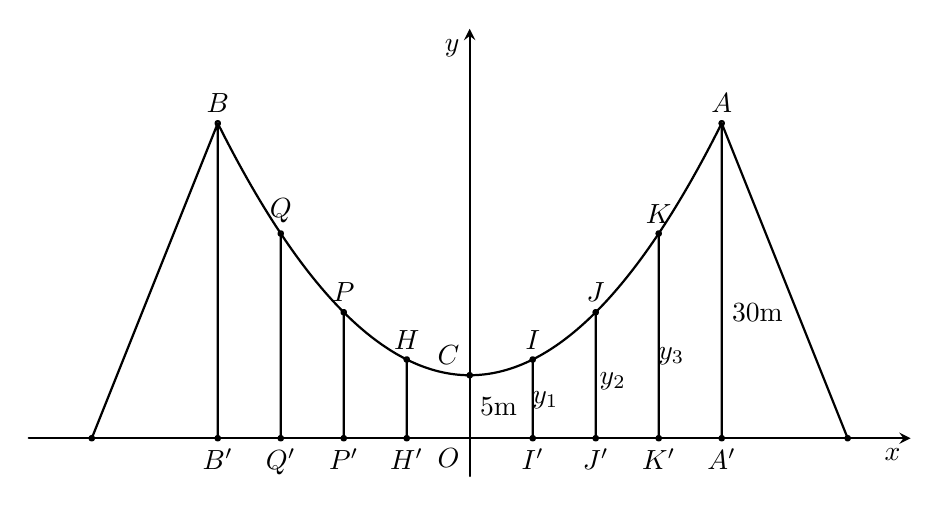
\begin{tikzpicture}[line join=round, line cap=round,>=stealth,thick,scale=.8]
\tikzset{label style/.style={font=\footnotesize}}
\draw[->] (-7,0)--(7,0) node[below left] {$x$};
\draw[->] (0,-0.6)--(0,6.5) node[below left] {$y$};
\draw (0,0) node [below left] {$O$};
\draw (1,0)--(1,1.25) (-1,0)--(-1,1.25)
(-2,0)--(-2,2) (2,0)--(2,2) (-3,0)--(-3,3.25) (3,0)--(3,3.25)
(-4,0)--(-4,5) (4,0)--(4,5) (-6,0)--(-4,5) (6,0)--(4,5);
\draw (0,1) circle (1pt)node [above left] {$C$};
\draw (1,0) circle (1pt)node [below] {$I'$} (1,1.25) circle (1pt) node [above] {$I$};
\draw (0,.5) node [right] {$5$m} (1.2,.3) node [above] {$y_1$};
\draw (1.9,.9) node [right] {$y_2$} (3.2,1) node [above] {$y_3$};
\draw (4,2) node [right] {$30$m};
\draw (-1,0) circle (1pt)node [below] {$H'$} (-1,1.25) circle (1pt) node [above] {$H$};
\draw (-2,0) circle (1pt)node [below] {$P'$} (-2,2) circle (1pt) node [above] {$P$};
\draw (2,0) circle (1pt)node [below] {$J'$} (2,2) circle (1pt) node [above] {$J$};
\draw (-3,0) circle (1pt)node [below] {$Q'$} (-3,3.25) circle (1pt) node [above] {$Q$};
\draw (3,0) circle (1pt)node [below] {$K'$} (3,3.25) circle (1pt) node [above] {$K$};
\draw (-4,0) circle (1pt)node [below] {$B'$} (-4,5) circle (1pt) node [above] {$B$};
\draw (4,0) circle (1pt)node [below] {$A'$} (4,5) circle (1pt) node [above] {$A$};
\draw (-6,0) circle (1pt) (6,0) circle (1pt);
\begin{scope}
\clip (-4,-1) rectangle (4,6);
\draw[samples=200,domain=-4:4,smooth,variable=\x] plot (\x,{0.25*(\x)^2+1});
\end{scope}
\end{tikzpicture}
\end{center}
\begin{itemize}
\item Giả sử Parabol có dạng: $y=a{x^2}+bx+c,a \ne 0$.
\item Chọn hệ trục $Oxy$ sao cho $C' \equiv O$ như hình vẽ.
\item Khi đó parabol đi qua điểm $A(100;30)$ và có đỉnh $C(0;5)$.
\item Đoạn $A'B'$ chia làm $8$ phần, mỗi phần $25$ m.\\
Suy ra $\heva{
30&=10000a+100b+c \\
\dfrac{-b}{2a}&=0 \\
5&=c} $
$\Leftrightarrow \heva{
a&=\dfrac{1}{400} \\
b&=0 \\
c&=5 }$ $\Rightarrow (P) \colon y=\dfrac{1}{400}{x^2}+5.$
\item Khi đó, tổng độ dài của các dây cáp treo bằng\\
$\begin{aligned}
OC+2y_1+2y_2+2y_3&=5+2\left( \dfrac{1}{400}\cdot {{25}^2}+5 \right)+2\left( \dfrac{1}{400}\cdot {{50}^2}+5 \right)+2\left( \dfrac{1}{400}\cdot {{75}^2}+5 \right)\\ &=\dfrac{315}{4}\approx 78{,}8 \text{ m}.
\end{aligned}$
\end{itemize}
}
\end{ex}